\subsection{Vorteile von Angular [M]}
\setauthor{Fabian Maar}
Folgende Aspekte sprechen für die Nutzung von Angular in diesem Projekt:

\begin{itemize}
  \item Die Möglichtkeit der komponentenbasiertes Programmierung um komplexe Benutzeroberflächen übersichtlich zu unterteilen (siehe \ref{components}) 
  \item Die einfache und übersichtliche Einbindung von Libraries durch ngModules (siehe \ref{sec:NgModules} )
  \item Isolierung der Logik mit der Benutzeroberfläche durch die Model-View-Controller Architektur und die Model-View-ViewModel Architektur (siehe \ref{fig:tech:front:mvc-architecture} )
  \item 
  Dependency Injection für die Verbindung von Front-End zum Back-End (siehe \ref{DPI})
\end{itemize}

\subsubsection{Angular [M]}
\setauthor{Fabian Maar}
\begin{wrapfigure}{r}{0.3\textwidth}
  \begin{center}
    
\includegraphics[width=0.2\textwidth]{pics/AngularLogo.png}
   \caption{Angular Logo}
  \end{center}
\end{wrapfigure}
Angular ist ein Framework für Webapplikationen, das auf der Programmiersprache Typescript basiert. Es ist eines der renommiertesten Frameworks zur Front-End-Entwicklung, wird als Open-Source-Software zur Verfügung gestellt und besitzt somit eine große Community. So zählte es 2022 zu den zweitbeliebtesten Front-End Framework \cite{AngularEvidence} und wird von Milliardenkonzernen wie zum Beispiel Google oder PayPal verwendet. 
\cite{AngularEvidence2}

Die große Stärke von Angular ist die Erstellung von Single-Page-Applikationen, da es eine komponentenbasierte Struktur besitzt. Das bedeutet, der Code ist wiederverwendbar und verkapselt. Komplexe Logiken werden auf ihre Grundelemente reduziert und beeinflussen sich nicht gegenseitig. \cite{AngularGeneral}


Angular basiert auf dem Konzept des Model-View-Controller- (MVC) und Model-View-ViewModel (MVVM) Architecture Patterns. Diese Patterns werden verwendet, um die Logik von der Benutzeroberfläche zu trennen und komplexe Aufgaben einfacher zu bewältigen. Dies wird in der Fachsprache auch oft als \emph{Seperation of Concerns} bezeichnet.
\cite{AngularArchitecturePattern} 

Architecture Patterns sind Muster, die verwendet werden, um
\begin{itemize}
  \item eine Software-Anwendung zu strukturieren.
  \item die Redundanz von wiederholenden Code-Teile zu vermeiden.
  \item immer wiederkehrende Probleme durch eine einmalige Lösungen zu beheben.
  \item die Wartung und Testung zu erleichtern.
  \item Änderungen am Umfang und der Größe der Applikation leichter handhaben zu können. \cite{MVCmdn, MVVM, MVC}
\end{itemize} 

\paragraph{Model-View-Controler (MVC)}
Die \emph{Seperation of Concerns} wird bei diesem Pattern durch die Aufteilung der Applikation in Model, View und Controller realisiert. Dadurch ist es möglich, sich auf einen Aspekt der Implementierung zu fokussieren. 

\begin{figure} [h t]
  \centering
  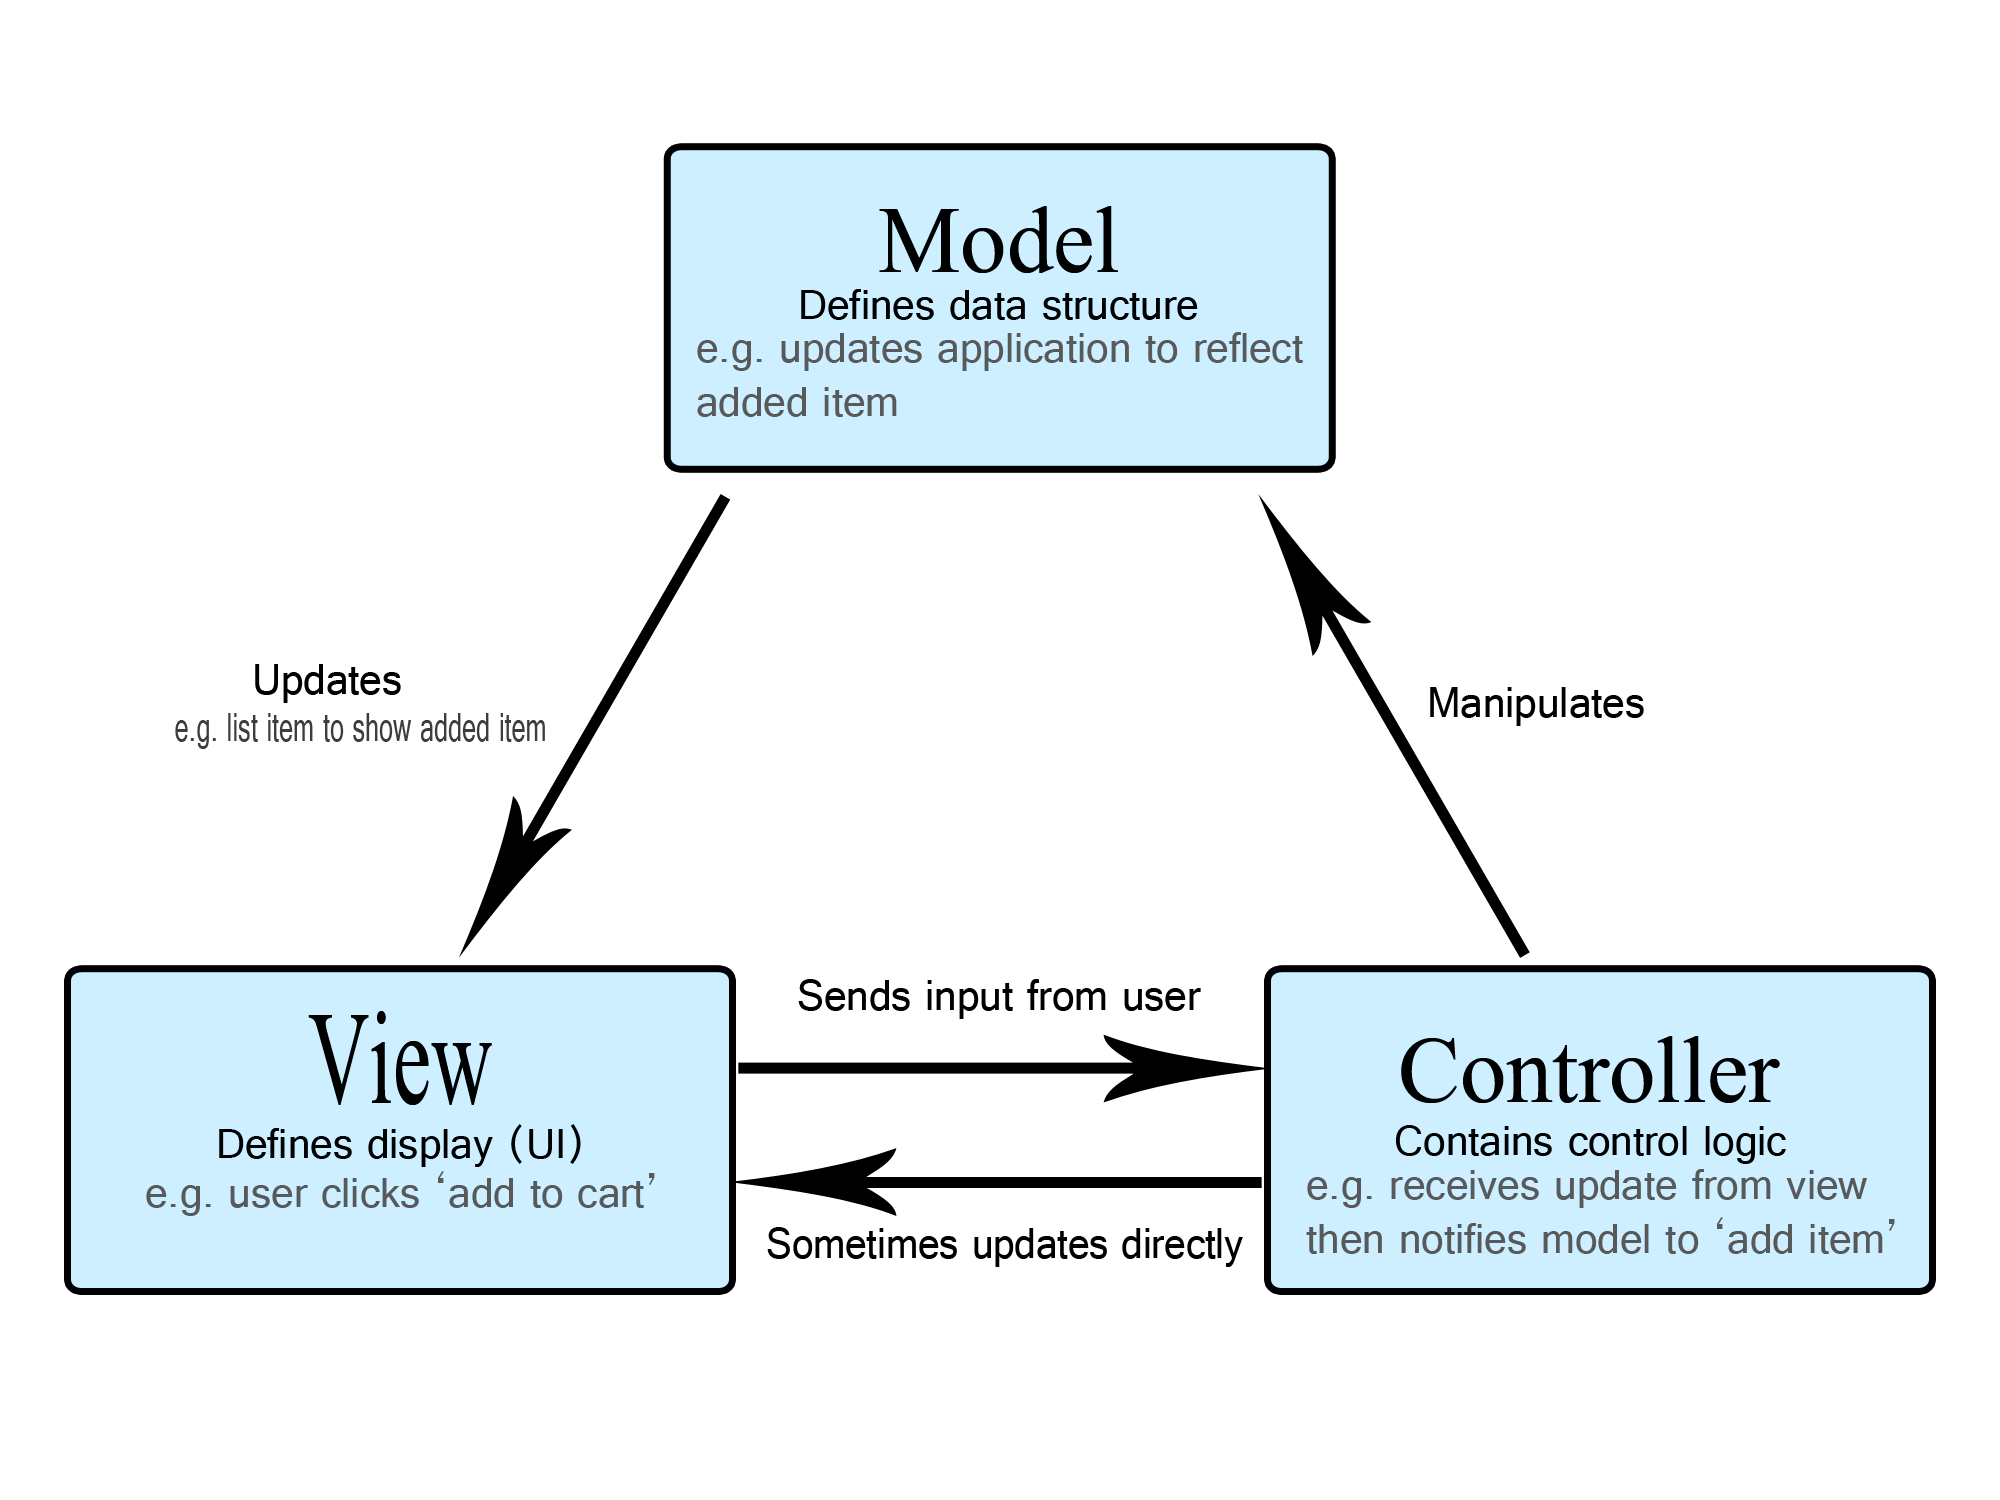
\includegraphics[scale=0.5]{pics/mvc.png}
  \caption{Die Model-View-Controller Pattern \cite{MVCmdn}}
  \label{fig:tech:front:mvc-architecture}
\end{figure}

Welche Daten eine Applikation beinhalten soll, wird über das Model geregelt. Falls sich das Model ändert, werden die Benutzerfläche und manchmal auch der Controller entsprechend geändert. In Angular sind diese Modelle mit den Interfaces (siehe Interfaces \ref{interface})  zu vergleichen.

\emph{View} ist die Benutzeroberfläche des Programms. Der*die Benutzer*in kann mit dieser interagieren und diese verändern. Sie wird aus den Daten des Models erstellt und definiert. In Angular kann diese View mit dem HTML-Template einer Komponente verglichen werden.

Im Controller werden die Eingaben der Benutzer*innen verarbeitet und die betroffenen Model- und View-Komponenten beeinflusst und verändert. Auch ist es möglich zu bestimmen, welche Views verändert werden sollen um die Daten gegebenenfalls in unterschiedlichen Formaten anzuzeigen. Die TypeScript-Files in Angular sind vergleichbar mit diesen Controllern.
\cite{MVC}

\paragraph{Model-View-ViewModel (MVVM)}
Das MVVM basiert auf dem Konzept des MVC-Patterns und realisiert die \emph{Seperation of Concerns} durch die View, ViewModel und Model Komponenten.

\begin{figure} [h t]
  \centering
  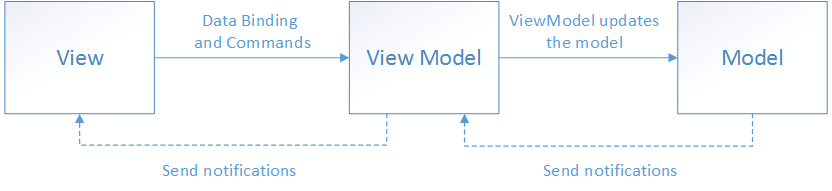
\includegraphics[scale=0.5]{pics/mvvm-pattern.png}
  \caption{Die Model-View-ViewModel Pattern \cite{MVVM}}
  \label{fig:tech:front:mvvm-architecture}
\end{figure}

\emph{View} funktioniert hierbei ähnlich wie beim MVC-Pattern, jedoch ist es möglich, dass eine \emph{View} auch Logik enthält, die Änderungen am Aussehen durchführt. Daher ist das HTML-Template einer Angular-Komponente noch stärker vergleichbar zu dem Konzept einer View aus dem MVVM-Pattern als zu einer View aus dem MVC-Pattern. 

Im ViewModel wird die Funktionalität der Benutzeroberfläche bestimmt. Dabei informiert das ViewModel die View über Änderungen im Model und beliefert es mit Daten. Dieser Vorgang beschreibt das Konzept des Data-Bindings (siehe \ref{data-binding}) in Angular.  

Das Model funktioniert im Grunde gleich wie beim MVC-Pattern, nur wird hierbei nicht die View, sondern das ViewModel über Änderungen informiert. Somit ist das ViewModel das Mittelstück zwischen View und Model.

Angular nutzt hierbei eine Mischung aus beiden Architecture-Patterns. Diese Architektur wird durch das Konzept von Komponenten realisiert. In den nächsten Kapiteln, besonders im Kapitel Umsetzung der Landingpage \ref{landingpage implentation} wird näher darauf eingegangen. Dabei werden die Parallelen der Patterns erkennbar.
\cite{MVVM}

\paragraph{NgModules [M]}\label{sec:NgModules}
\setauthor{Fabian Maar}
\emph{NgModules} erleichtern die Einbindung von Libraries. Da keine externen Dateien mühsam heruntergeladen und eingebunden werden müssen und jeder Import-Prozess durch wenige Zeilen Code erfolgt, wird Zeit beim Entwickeln gespart. Alle Importe werden in chronologischer Reihenfolge gelistet, wodurch ein guter Gesamtüberblick geliefert wird und schnell überflüssige Imports entfernt werden können. Die kontinuierliche Erweiterung und die Unterstützung von Third-Party-Libraries, die unter anderem für die 3D-Darstellung verwendet werden, wird ebenfalls von diesen ngModulen ermöglicht. Die Angular-Applikation wird hierbei organisiert und gestartet, in dem die Metadaten wie folgt abgespeichert werden:

\begin{itemize}
  \item Declarations - In dieser Sektion werden alle zugehörigen Komponenten, Direktiven und Pipes deklariert. 
  \item Providers - Sie initialisieren wie die Werte bei der Dependency Inection (siehe \ref{DPI}) abgerufen werden. \cite{AngularProviders}
  \item Imports - Hier werden alle Libraries und exportierte Modules importiert.
  \item Exports - Sie beinhalten alle zu exportierenden Module
  \item Bootstrap - Hierbei wird angegeben welche Komponente beim Anwendungsstart zuerst geladen wird
\end{itemize}

Die Verwendung von ngModules in der 3D-Gallerie-Applikation wird im Abschnitt Routing (siehe Routing \ref{lst:impl:routing}) nochmals erklärt.
\cite{AngularNgModules}
\cite{AngularNgModulesAPI}
\cite{AngularBuch}


\subsubsection{Angular Schlüsseltechnologien [L]}
Angular ist ein hoch anpassbares Framework. Bei der Verarbeitung von asynchronen Prozessen und Events kann Angular um die Library RxJS erweitert werden. Bei der Paketierung und beim Update von geändertem Code wird der Entwickler von der Libary Webpack unterstützt. 

\setauthor{Litzlbauer Lorenz}
\paragraph{RxJS [L]}
\label{RxJS}
\begin{wrapfigure}{r}{0.3\textwidth}
  \begin{center}
    
\includegraphics[width=0.2\textwidth]{pics/RxJs_logo.png}
   \caption{RxJS Logo}
  \end{center}
\end{wrapfigure}
RxJS ist eine Implementierung von ReactiveX für die Programmiersprache Javascript.

ReactiveX ist eine Library für das Erstellen von asynchronen und eventbasierten Programmen, dafür benutzt es \emph{observable sequences}. Ein beobachtetes Subjekt führt eine Liste von den Observern. Bei einer Veränderung im Subjekt werden die Beobachter nach der Reihenfolge der Liste über die Veränderung informiert (siehe \ref{txt:glos:observerDesignPattern}).
Die Library arbeitet mit dem \emph{Observer-Design-Pattern} und fügt verschiedene neue Operatoren hinzu. Zusätzlich werden Low-Level-Funktionen wie Threading, Synchronisation und Thread-Sicherheit verarbeitet und keine Input-/Output-Prozesse blockiert. \cite{ReactiveXIntro}

\paragraph{Webpack [L]}
\begin{wrapfigure}{r}{0.3\textwidth}
  \begin{center}
    
\includegraphics[width=0.2\textwidth]{pics/webpack-logo.png}
   \caption{Webpack Logo}
  \end{center}
\end{wrapfigure}
Die Hauptfunktion von Webpack ist es, viele verschiedene Daten zu einem Paket für eine JavaScript Applikation zusammenzufassen.
Angular benutzt Webpack, um TypeScript in JavaScript und SASS bzw. SCSS in CSS umzuwandeln. Beim Bauen des Projektes werden alle Module in ein einziges zusammengefasst. Bei der Entwicklung der Applikation wird durch Webpack \emph{Live-Reloading} unterstützt. Dabei wird bei einer Änderung im Code die gesamte Applikation aktualisiert und neu gestartet. \cite{Webpack}

\subsection{User-Interface-Frameworks (UI-Frameworks) [L]}
Ein User-Interface-Framework ist eine Ansammlung von Web Komponenten wie beispielsweise einer Navigationsleiste, die sofort im Projekt nutzbar ist. \cite{CssFrameworkExplaination}


Die Vorteile von UI-Frameworks sind:
\begin{compactitem}
    \item Sie vereinfachen und beschleunigen den Entwicklungsprozess. Typische Web-Komponenten Web-Komponenten sind vordefinierte, der Entwickler muss diese nicht mehr implementieren und erspart sich Zeit. \cite{BestCSSFrameworksin2022}
    \item Sie achten bei den Komponenten und Styling-Features darauf, dass diese auch auf allen Internet-Browser angezeigt werden können.
    Besonders bei neuen CSS-Feature kann es sein, dass diese noch nicht von allen Browsern unterstützt werden. Ein UI-Framework benutzt in der Regel nur Funktionen, die auch alle Browser anzeigen können. \cite{CssFrameworkExplaination}
    \item Der Code hat eine bessere Lesbarkeit.
    In einem UI-Framework gibt es gewisse Konventionen wie Klassennamen, die befolgt werden müssen. Dadurch wird der Code besser lesbar. \cite{CssFrameworkExplaination}
\end{compactitem}


Die Nachteile von UI-Frameworks sind: 
\begin{compactitem}
    \item Die Ladezeit der Webseite erhöht sich;
    Schließlich müssen auch mehr Daten an den Browser geschickt werden.
    \item Webseiten, die das selbe UI-Framework verwenden, weisen visuelle Ähnlichkeiten auf, da die Web-Komponenten gleich implementiert wurden.
\end{compactitem}


\subsection{UI-Frameworks im Projekt [L]}
Im Projekt werden die beiden UI-Frameworks, \emph{Bootstrap} und \emph{AngularMaterials} verwendet.


\subsubsection{Angular Material [L]}
\begin{wrapfigure}{r}{0.3\textwidth}
  \begin{center}
    
\includegraphics[width=0.2\textwidth]{pics/Angular_Material_UI_Logo.png}
   \caption{Angular Material UI Logo}
  \end{center}
\end{wrapfigure}
\emph{Angular Material} ist eine UI Framework und wird seit 2014 von Google entwickelt. Das Framework baut auf Angular auf und erweitert es mit eigenen Komponenten, Styleguides, Typographie und vielem mehr. Die Design-Sprache orientiert sich dabei an der \emph{Material Design Spezifikation} von Google. Ein großer Fokus des Frameworks liegt in der Responsivität. \cite{JavaPointAngularMaterial, WhatAngularMaterial}


\emph{Angular Material} bietet folgende Features: 
\begin{compactitem}
    \item Erweiterbar: bei der Installation lassen sich viele Designanpassungen machen, zusätzlich lassen sich Styles mit dem globalen Stylesheet überschreiben. \cite{JavaPointAngularMaterial}
    \item Hochwertig: die Komponenten sind erprobt und wurden auf die Performanz und Verlässlichkeit getestet. \cite{JavaPointAngularMaterial}
    \item Reibungslos: Angular Material ist einzig und allen für Angular als UI-Library entwickelt worden.\cite{JavaPointAngularMaterial}
\end{compactitem}

Angular Material bietet eine hohe Anzahl an sofort einsetzbaren Komponenten. Zu all diesen Komponenten gibt es auf der offiziellen Webseite eine ausführliche Dokumentation mit Beispielen. \cite{JavaPointAngularMaterial, WhatAngularMaterial}

\paragraph{Material Design Spezifikation [L]}
\emph{Material Design} ist ein Styleguide der von der Firma Google entwickelt wurde. Er soll dabei helfen, qualitative hochwertige digitale Produkte für Android, iOS, Flutter und das Web zu gestalten.

\emph{Material Design} befolgt für die Design-Richtung mehrere Prinzipien. 

\emph{Material Design} soll die reale Welt abbilden.
Durch Typographie, Raster, Abstände, Farben und Bilder soll eine erkennbare Hierarchie entstehen. Die Komponenten dienen als interaktive Bauklötze. Komponenten haben alle ein Stati-System, welches den Status der Komponente fokussiert, selektiert, aktiviert, fehlerhaft, schwebend, gedrückt und/oder deaktiviert anzeigt. Durch mehrere vordefinierte Themes ist es möglich einzelne Komponenten zu verändern und das Design so anzupassen, dass es zur Corporate Identity der*des Benutzer*in passt.\cite{MaterialDesign-Introduction}

\paragraph{Angular Material Komponente im Projekt [L]}

\begin{figure}
  \centering
  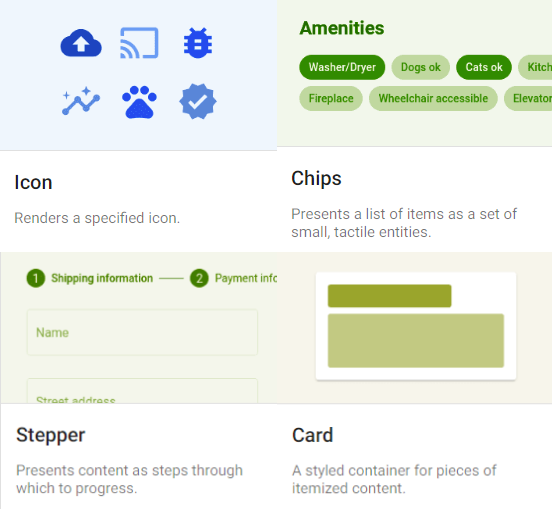
\includegraphics[scale=0.5]{pics/AngularMaterialKomponent.png}
  \caption{Angular Material: Komponenten die im Projekt verwendet wurden \cite{AngularComponents}}
  \label{architecture:frontend:angular-material-project-components}
\end{figure}

Im Projekt wurden hauptsächlich die Angular Material Komponenten \emph{mat-icon}, \emph{mat-chips}, \emph{mat-stepper} und \emph{mat-chard} verwendet (siehe Abbildung \ref{architecture:frontend:angular-material-project-components}).

{mat-icon} wird dafür verwendet, die Icons auf der Single-Page-Application anzuzeigen. Angular Material besitzt eine Icon-Library. Wenn \emph{mat-icon} verwendet wird, wird durch den Inhalt des \emph{mat-icon}-Tags das Icon dynamisch aus der Icon-Library geladen.

\emph{mat-chips} werden für das Design der Ausstellungskriterien benützt. Sie kommen in der Content-Creation und der Suchseite vor.

\emph{mat-stepper} wird bei der Content-Creation verwendet, um die Wizard-Funktion umzusetzen.

\emph{mat-chard} wird für die Ausstellungsstückkarten auf der Single-Page-Application verwendet. Diese kommen auf der Profile-, Such- und Landing-Page vor.

\subsubsection{Bootstrap [L]}
\begin{wrapfigure}{r}{0.3\textwidth}
  \begin{center}
    
\includegraphics[width=0.2\textwidth]{pics/Bootstrap_logo.png}
   \caption{Bootstrap Logo}
  \end{center}
\end{wrapfigure}
Bootstrap ist ein kostenloses Open-Source-Frontend-Framework. Es fungiert als eine Art Bibliothek mit zahlreichem HTML sowie CSS Gestaltungsvorlagen. Auch die Integration von JavaScript ist durch Bootstrap möglich. Es bietet mehrere Komponenten an. Ziel von Bootstrap ist es den*der Entwickler*in das Umsetzen von interaktive und responsive Webseiten zu erleichtern. \cite{BestCSSFrameworksin2022}

Bootstrap beinhaltet folgenden Features:  
\begin{compactitem}
    \item Web-Komponenten, die sofort anwendbar sind \cite{BestCSSFrameworksin2022} 
    \item eine gute Dokumentation \cite{BestCSSFrameworksin2022}
    \item Mobile Centered Design \cite{BestCSSFrameworksin2022}
    \item hohe Benutzerfreundlichkeit \cite{BestCSSFrameworksin2022}
\end{compactitem}

\subsubsection{SCSS [L]}
\begin{wrapfigure}{r}{0.3\textwidth}
  \begin{center}
    
\includegraphics[width=0.2\textwidth]{pics/Sass_Logo.png}
   \caption{Sass Logo}
  \end{center}
\end{wrapfigure}
SCSS ist eine Syntax- und Feature-Erweiterung von CSS, und bietet folgende Vorteile:

\begin{compactitem}
  \item Variablen \cite{SassGuide}
  \item Schleifen \cite{SassGuide}
  \item Kalkulationen \cite{SassGuide}
  \item Mixins \cite{SassGuide}
  \item Imports \cite{SassGuide}
  \item Verschachtelung \cite{SassGuide}
\end{compactitem}

Besonders ausschlaggebend für die Auswahl von SCSS war das Prinzip der Verschachtelung. Durch die Verschachtelung kann an redundanten Selektoren gespart werden, was die Style-Definition besser lesbar macht. In den angeführten Beispielen (siehe SCSS-Code-Beispiel \ref{lst:imp:design:scss} und natives CSS-Code-Beispiel \ref{lst:imp:design:css}) werden die Schreibweisen von SCSS und CSS gegenübergestellt dargelegt. \cite{SassGuide}

\begin{lstlisting}[caption=SCSS - Code Beispiel \cite{SassGuide},label=lst:imp:design:scss]
nav {
    ul {
        margin: 0;
        padding: 0;
        list-style: none;
    }
    
    li { display: inline-block; }
    
    a {
        display: block;
        padding: 6px 12px;
        text-decoration: none;
    }
}
\end{lstlisting}

\begin{lstlisting}[caption=CSS - Code Beispiel \cite{SassGuide},label=lst:imp:design:css]
nav ul {
    margin: 0;
    padding: 0;
    list-style: none;
    }
nav li {
    display: inline-block;
    }
nav a {
    display: block;
    padding: 6px 12px;
    text-decoration: none;
}
\end{lstlisting}

Die Syntax- und Feature-Erweiterung haben uns dazu veranlasst, SCSS im Projekt einzusetzen.


\subsection{3D Rendering [L]}
Es gab verschiedene Auswahlkriterien für die benötigte 3D-Web-API, die ausschlaggebend für den Projekterfolg waren:
\begin{compactitem}
  \item Effizienzen der 3D Engine (Hardware Acceleration, RAM-Auslastung)
  \item Benutzerfreundlichkeit (Developer-Experience)
  \item Das Laden von 3D-Modellen aus 3D-Dateien und aus dem Internet
  \item Unterstützung von Video-Texturen
\end{compactitem}

\subsubsection{Three.js [L]}
\setauthor{Litzlbauer Lorenz}
\begin{wrapfigure}{r}{0.3\textwidth}
    \begin{center}
      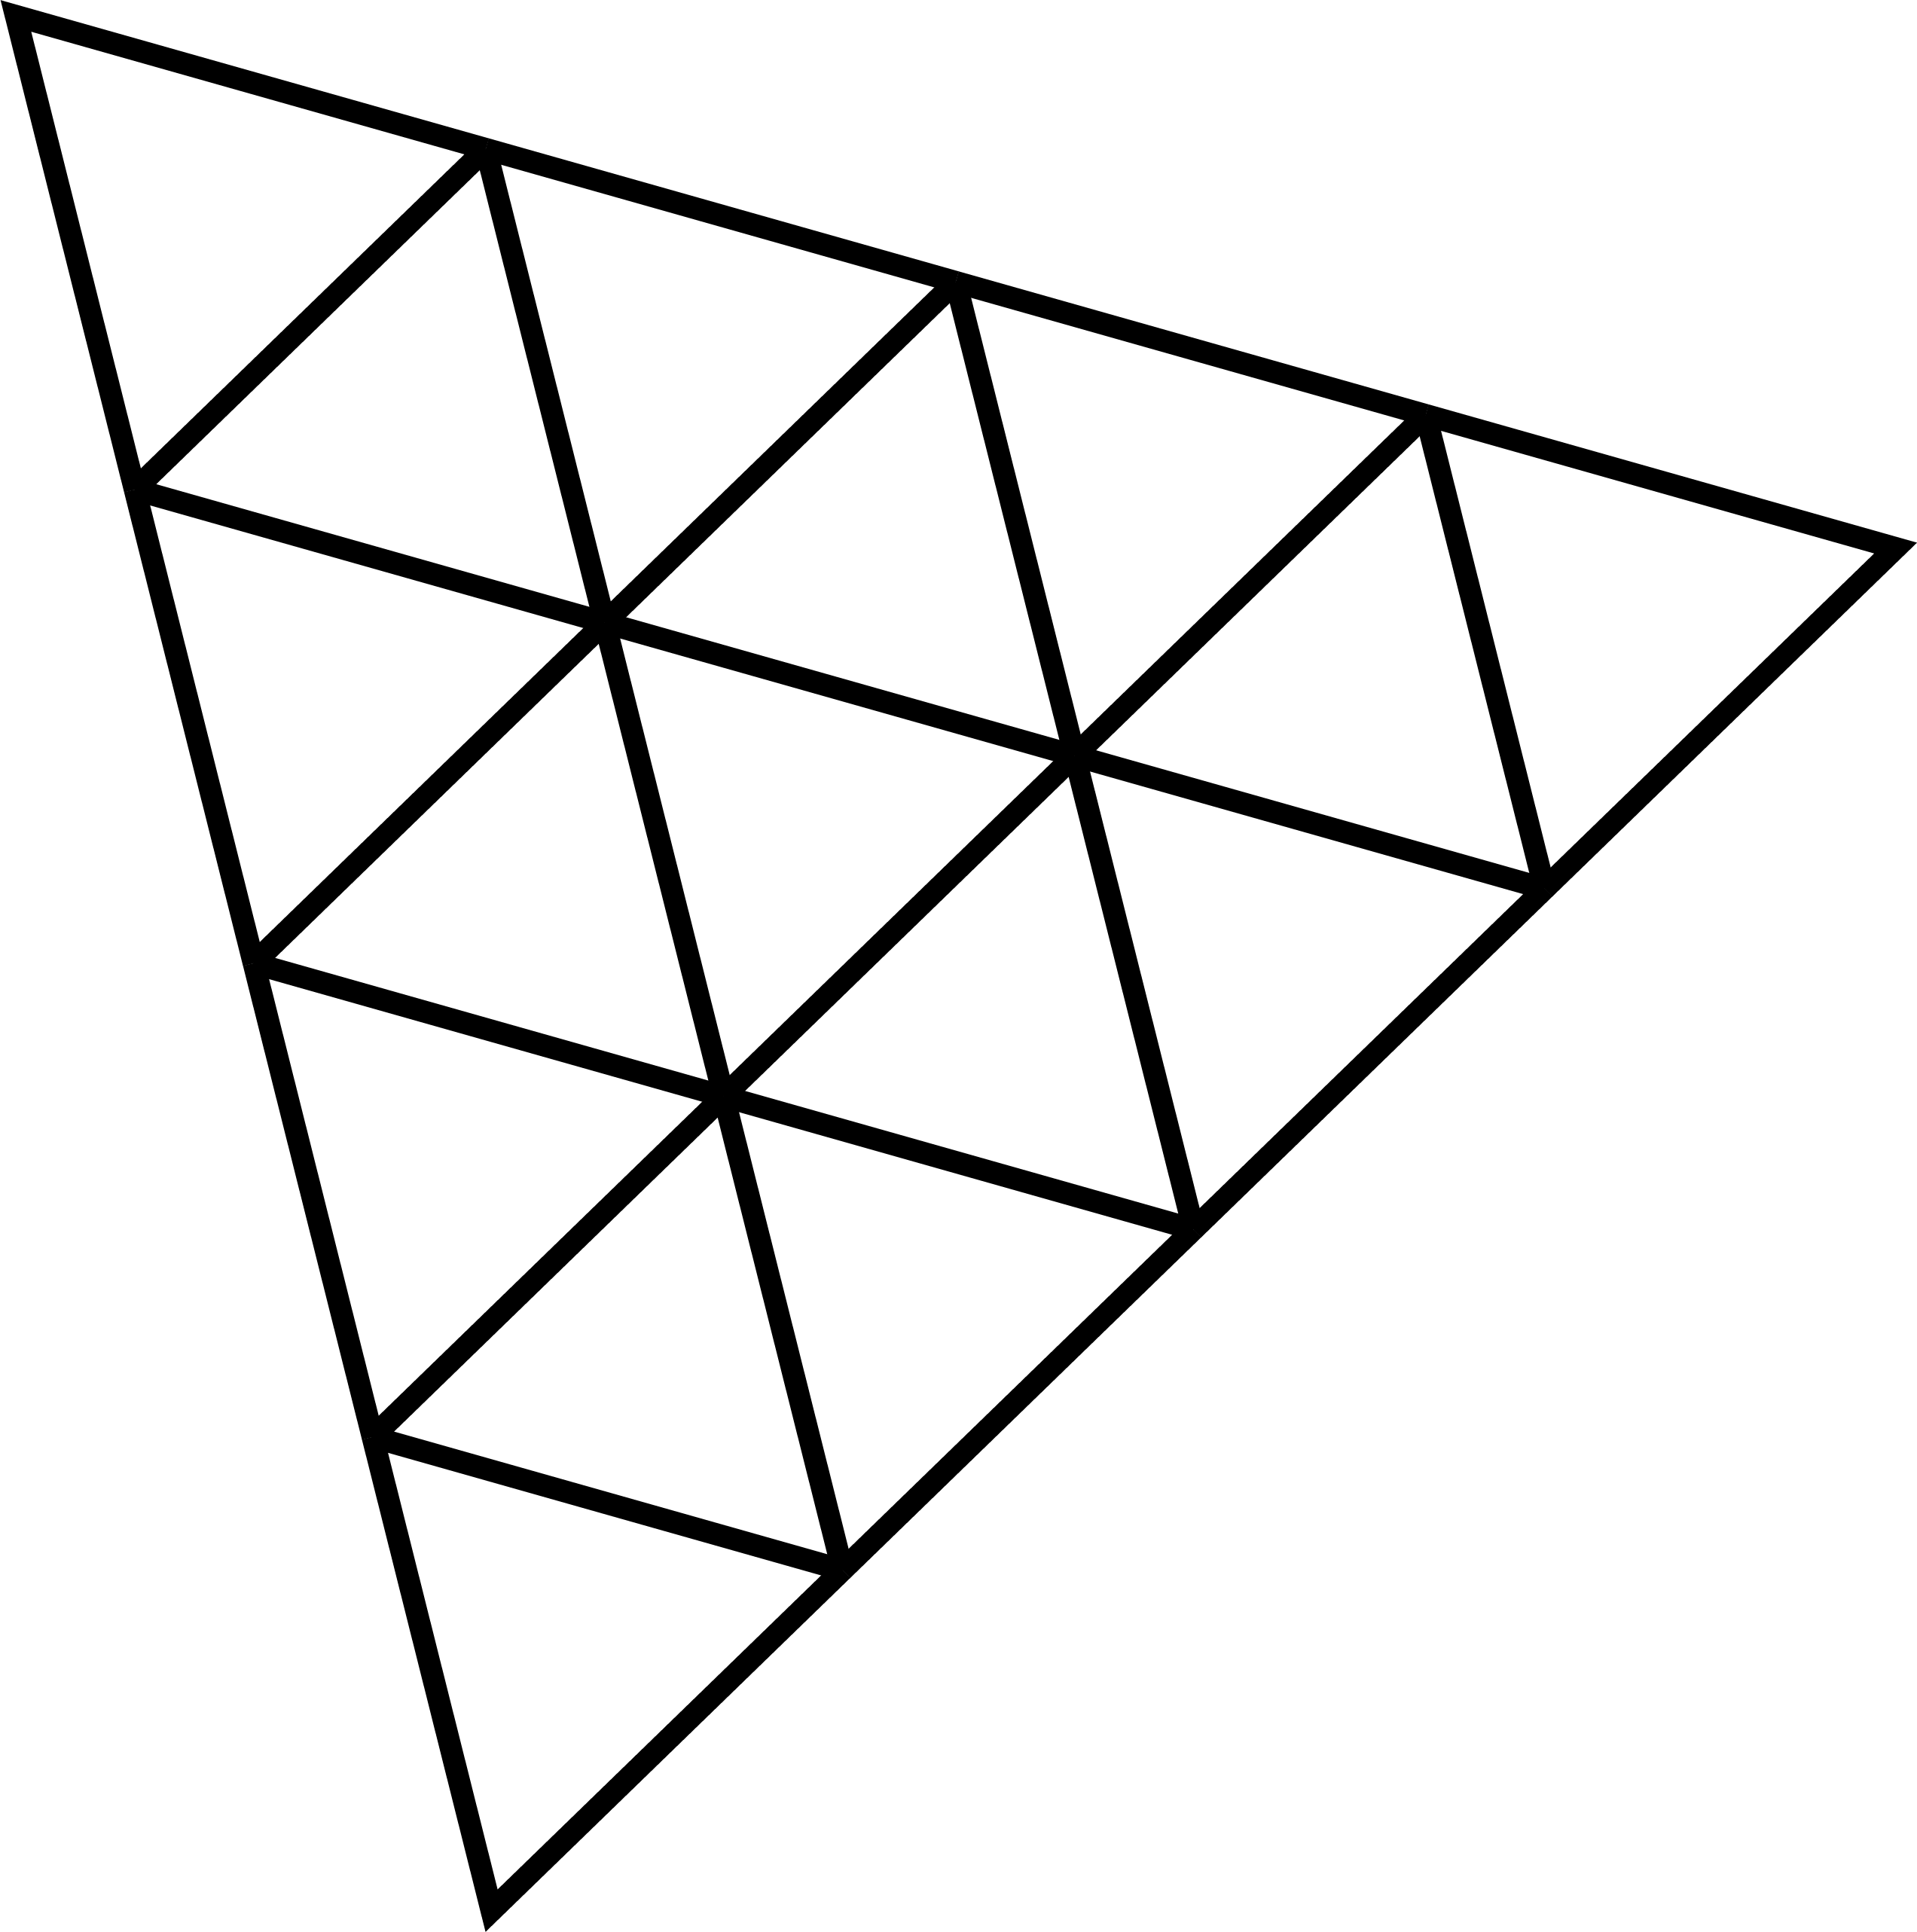
\includegraphics[width=0.2\textwidth]{pics/threeJS.png}
     \caption{Three.js Logo}
    \end{center}
\end{wrapfigure}
\emph{Three.js} ist eine JavaScript Library für die Darstellung von 3D-Grafiken im Web. Für die 3D-Darstellung nutzt Three.js WebGL (mehr dazu im nächsten Abschnitt \hyperref[ch::webgl]{WebGL}), ein Low-Level-Framework. WebGL hat eine hohe Komplexität. Three.js bietet eine Abstraktion von WebGL, um Anwendungen für 3D-Webanwendungen für Entwickler zugänglicher zu machen.
Three.js regelt Systeme wie die 3D-Szene, Lichter, Schatten, Materialien, Texturen und 3D-Matrix-Rechnungen, deren Umsetzung mittels WebGL sehr aufwändig wäre. \cite{ThreeJsFund}

\begin{figure} [h t]
  \centering
  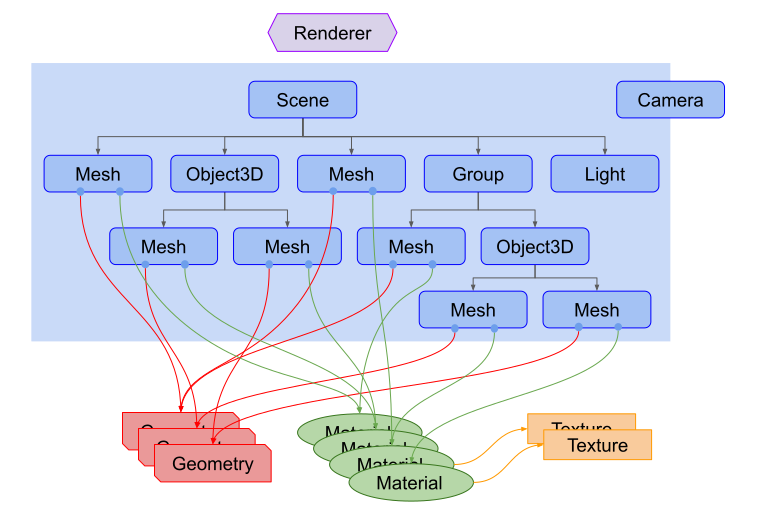
\includegraphics[scale=0.5]{pics/threejs-structure.png}
  \caption{Die Struktur von Three.js \cite{ThreeJsFund}}
  \label{fig:tech:front:threejsstructure}
\end{figure}

In Three.js werden Geometrie, Objekte und Materialien verbunden, um ein 3D-Objekt zu erstellen. 
Die Abbildung \ref{fig:tech:front:threejsstructure} veranschaulicht den beispielhaften Aufbau eines solchen Objektes. In diesem Objekt werden Meshes, Gruppen, Lichter und 3D-Objekte in einer Baumdatenstruktur gesammelt. Die Daten über die Geometrie sowie Materialien der Meshes werden außerhalb der Szene gespeichert und die Meshes referenzieren im Renderprozess darauf. \cite{ThreeJsFund}

\paragraph{WebGL [L]}
\label{ch::webgl}
\label{ch::ThreeJsDependency}
\begin{wrapfigure}{h  r}{0.3\textwidth}
    \begin{center}
      
\includegraphics[width=0.2\textwidth]{pics/WebGL_Logo.png}
     \caption{WebGL Logo}
    \end{center}
\end{wrapfigure}
WebGL ist eine lizenzfreie Low-Level-API, die dafür benutzt wird, 3D-Grafiken im Web darzustellen. Sie basiert auf OpenGL ES 2.0 und benutzt auch dieselbe Grafik-Programmiersprache, wie Open GLSL (OpenGL Shading Language). Eine Low-Level-API hat einen höheren Konfigurierungsgrad und lässt sich für spezielle Anwendungsfälle besser anpassen. Die API setzt ein viel tieferes Verständnis von dem Material (WebGL Shader-Programmierung, Matrixrechnungen usw.) voraus und bringt somit einen höheren Programmieraufwand mit sich. \cite{WebglGettingStarted, HighlowAPI}

\subsubsection{Weitere Web Rendering APIs [L]}
Es gibt viele weitere Technologien, die 3D-Grafiken im Web ermöglichen, wie beispielsweise Babylon.js, A-Frame, X3DOM und WebGL.

\paragraph{A-Frame [L]}
\emph{A-Frame} wird von der \emph{Mozilla Foundation} als OpenSource-Projekt entwickelt. Die 3D-Szene wird durch eine deklarative Sprache mit XML-Syntax definiert. Über die WebVR-API bietet die Libray auch die Möglichkeit, 3D-Szenen durch eine VR-Brille zu erfahren. \cite{a-frame-wiki}

A-Frame hat ähnliche Funktionen und Leistung im Vergleich zu Three.js. A-Frame sticht besonders bei der VR-Unterstützung hervor. Doch wird dieses Feature nicht im Projekt gebraucht. A-Frame baut auf Three.Js auf und erweitert es. Dadurch steigt die Komplexität, deswegen wird sich im Projekt gegen die Verwendung von A-Frame entschieden. \cite{a-frame-wiki}

\subsubsection{Angular Three [L]}
\label{ch:Technologien:AngularThree}
\emph{Angular Three} ist ein Open Source Projekt von Matt DesLauriers. Es zielt darauf ab die Vorteile von Angular und Three.js zu kombinieren. Dabei verbindet es das Prinzip der Komponenten von Angular mit der 3D Darstellung von Three.js. 

\begin{lstlisting}[language=html,caption=Angular Three - Komponentenbasiertes 3D Scenen in HTML  \cite{AngularThreeDocumentationFirstScene},label=lst:impl:AngularThreeExampleCode]
<ngt-canvas>
    <ngt-ambient-light intensity="0.5"></ngt-ambient-light>
    <ngt-spot-light [position]="10" angle="0.15" penumbra="1"></ngt-spot-light>
    <ngt-point-light [position]="-10"></ngt-point-light>
  
    <app-cube [position]="[1.2, 0, 0]"></app-cube>
    <app-cube [position]="[-1.2, 0, 0]"></app-cube>
  
    <ngt-soba-orbit-controls></ngt-soba-orbit-controls>
</ngt-canvas>
\end{lstlisting}

\begin{lstlisting}[language=html,caption=Angular Three - App Cube  \cite{AngularThreeDocumentationFirstScene},label=lst:impl:AngularThreeCube]
<ngt-mesh
  (beforeRender)="onCubeBeforeRender($event)"
  (click)="active = !active"
  (pointerover)="hovered = true"
  (pointerout)="hovered = false"
  [scale]="active ? 1.5 : 1"
  [position]="position"
>
  <ngt-box-geometry></ngt-box-geometry>
  <ngt-mesh-standard-material [color]="hovered ? 'turquoise' : 'tomato'"></ngt-mesh-standard-material>
</ngt-mesh>
\end{lstlisting}
Angular Three ermöglicht eine schnelle und einfache Erstellung einer 3D-Szene. Die 3D-Abbildung kann durch nur wenige Zeilen Code \ref{lst:impl:AngularThreeExampleCode} definiert werden. Die Business-Logik kann durch das komponentenbasierte Programmieren ausgelagert werden. Das wird durch das Codebeispiel App-Cube \ref{lst:impl:AngularThreeCube} verdeutlicht.  \cite{AngularThreeCode}

Ein weiterer Vorteil von Angular Three ist die ausführliche Dokumentation mit Codebeispielen. \cite{AngularThreeCode}

Angular Three bietet viele Vorteile: 
\begin{compactitem}
  \item hohe Benutzerfreundlichkeit
  \item ähnliche 3D-Leistung zu Three.js
  \item gute Integration mit Angular
  \item komponentenbasiert Programmieren
\end{compactitem}
Wegen den zahlreichen Vorteilen bietet sich die Library für das Projekt an.

Mithilfe eines Prototypen (siehe \hyperref[ch::ongoing-prototyping]{fortlaufendes Prototyping}) wurde getestet, ob Angular Three alle Features, die für das Projekt benötigt werden, unterstützt. Dabei wurde festgestellt, dass sich die Library Angular Three für das Projekt nicht eignet. 

Trotz der vielen Features konnten einige Kriterien für die Projektumsetzung wie das dynamische Laden von Objekten, komplexe Szenen und Interaktions- und Bewegungsarten im Prototypen nicht erfüllt werden. So wurden beispielsweise 3D-Objekte, wenn sie mehrere Male von einer lokalen Datei geladen werden, aufgrund von Problemen bei der Implementierung Angular Three's Caching nicht mehr angezeigt. Außerdem funktionierten Angular-Three-Module wie die FristPersonControls nicht.

Weil Angular Three nicht die für das Projekt aufgestellten Anforderungen erfüllt hat, wurde sich dafür entschieden, rein auf Three.js ohne weitere Abhängigkeiten zu setzen.

\paragraph{Angular Thee - Abgebrochene Entwicklung}
Das GitHub-\emph{Angular Three}-Repository wurde am 10. Februar 2023 archiviert. Der Source Code ist noch immer öffentlich zugänglich, doch gibt es keine Pläne, das Projekt weiterzuentwickeln. \cite{AngularTheeGithub} 

\subsection{Sicherheit [L]}
\setauthor{Litzlbauer Lorenz}

\subsection{JWT - Json Web Token [L]}
\begin{wrapfigure}{r}{0.3\textwidth}
  \begin{center}
    
\includegraphics[width=0.2\textwidth]{pics/jwt_logo.png}
   \caption{JWT Logo}
  \end{center}
\end{wrapfigure}
Der Json Web Token (JWT) ist ein offenerer Standard des Access-Token, der durch RFC 7519 definiert wird. JWT wird zur sicheren Übertragung von Informationen über ein JSON-Objekt benutzt, indem er den*die Benutzer*in authentifiziert. Die Authentifizierung passiert am Server. Dort wird nach einer Validierung erfolgt eine digitale Signatur des Token. Dies geschieht mittels Passwort oder eine Hashfunktion wie HMAC oder durch ein asymmetrisches Kryptosystem wie RSA. \cite{jwtAuth0}


